% Why an apex-independent axis is more robust: under the reference formula the measurement
% axis is re-estimated from the same perturbed landmarks it then projects, so landmark error
% has a ROTATION term. Under a mask-derived axis that term is identically zero.
\documentclass[border=8pt,multi,tikz]{standalone}
\usepackage{amsmath}
\usepackage{helvet}
\renewcommand{\familydefault}{\sfdefault}
\usetikzlibrary{positioning,arrows.meta,calc,angles,quotes,decorations.pathreplacing,
                decorations.markings,backgrounds,patterns}

\definecolor{ink}{HTML}{1D2433}
\definecolor{muted}{HTML}{6B7280}
\definecolor{accent}{HTML}{D62828}
\definecolor{good}{HTML}{2A9D8F}
\definecolor{cejc}{HTML}{0091C2}
\definecolor{intc}{HTML}{D99400}
\definecolor{apexc}{HTML}{B5179E}
\definecolor{tooth}{HTML}{DFE6EE}

\begin{document}
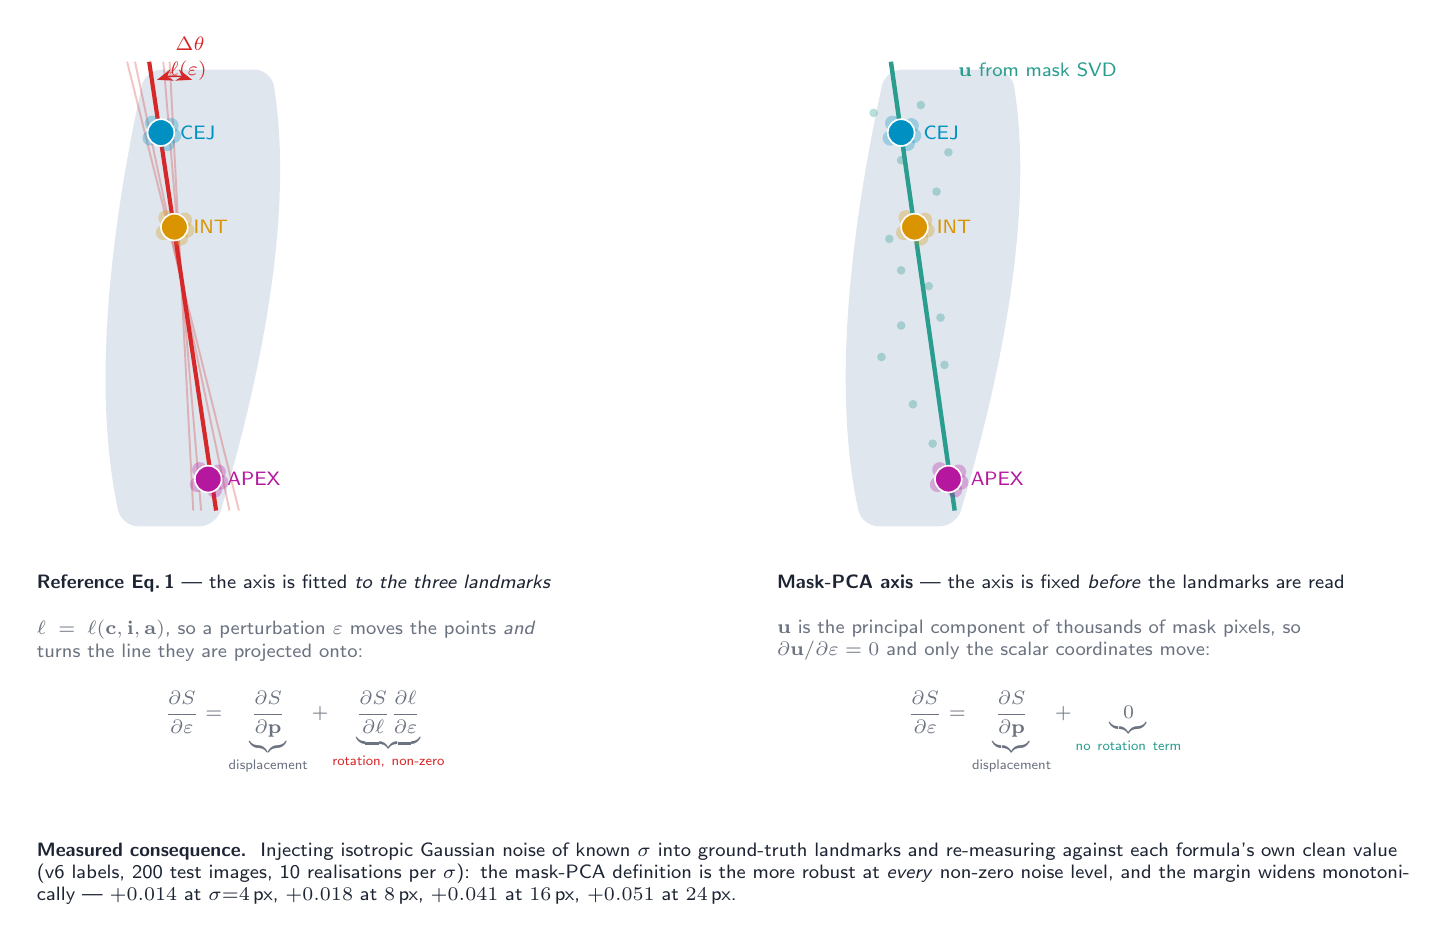
\begin{tikzpicture}[
  font=\sffamily\footnotesize,
  >={Stealth[length=2mm]},
  kp/.style={circle,draw=white,line width=0.6pt,minimum size=3.4mm,inner sep=0pt},
  ghost/.style={circle,fill opacity=0.30,minimum size=1.9mm,inner sep=0pt},
  lbl/.style={font=\sffamily\scriptsize,text=muted,align=center},
  note/.style={font=\sffamily\scriptsize,align=left},
]

%================================================================ LEFT PANEL ===
\begin{scope}[xshift=0cm]
  % tooth body
  \fill[tooth,rounded corners=6pt]
    (0.85,0.35) .. controls (0.45,2.2) and (0.75,4.3) .. (1.15,6.15) --
    (2.75,6.15) .. controls (3.05,4.3) and (2.6,2.2) .. (2.05,0.35) -- cycle;

  \coordinate (C)  at (1.35,5.35);
  \coordinate (I)  at (1.52,4.15);
  \coordinate (A)  at (1.95,0.95);

  % family of axes refitted from perturbed landmarks
  \draw[accent,opacity=0.28,line width=0.7pt] (1.02,6.25) -- (2.22,0.55);
  \draw[accent,opacity=0.28,line width=0.7pt] (1.38,6.25) -- (1.86,0.55);
  \draw[accent,opacity=0.28,line width=0.7pt] (0.92,6.25) -- (2.34,0.55);
  \draw[accent,opacity=0.28,line width=0.7pt] (1.46,6.25) -- (1.76,0.55);
  \draw[accent,line width=1.5pt] (1.20,6.25) -- (2.05,0.55) node[pos=0.02,right=1mm,
        font=\sffamily\scriptsize,text=accent]{$\ell(\varepsilon)$};

  % the rotation the family represents
  \draw[<->,accent,line width=0.6pt] (1.30,6.02) arc[start angle=108,end angle=72,radius=0.72];
  \node[font=\sffamily\scriptsize,text=accent] at (1.72,6.48) {$\Delta\theta$};

  \foreach \p/\c in {C/cejc,I/intc,A/apexc}{
    \foreach \dx/\dy in {0.13/0.09,-0.11/0.12,0.08/-0.14,-0.14/-0.07,0.16/-0.04}{
      \node[ghost,fill=\c] at ($(\p)+(\dx,\dy)$) {};}
  }
  \node[kp,fill=cejc]  (Cp) at (C) {};
  \node[kp,fill=intc]  (Ip) at (I) {};
  \node[kp,fill=apexc] (Ap) at (A) {};
  \node[font=\sffamily\scriptsize,text=cejc,right=1.2mm]  at (Cp) {CEJ};
  \node[font=\sffamily\scriptsize,text=intc,right=1.2mm]  at (Ip) {INT};
  \node[font=\sffamily\scriptsize,text=apexc,right=1.2mm] at (Ap) {APEX};

  \node[note,text=ink,anchor=north west] at (-0.35,-0.15)
    {\textbf{Reference Eq.\,1} --- the axis is fitted \emph{to the three landmarks}};
  \node[note,text=muted,anchor=north west,text width=68mm] at (-0.35,-0.72)
    {$\ell=\ell(\mathbf{c},\mathbf{i},\mathbf{a})$, so a perturbation $\varepsilon$ moves the points
     \emph{and} turns the line they are projected onto:
     \[\frac{\partial S}{\partial\varepsilon}
       =\underbrace{\frac{\partial S}{\partial \mathbf{p}}}_{\text{displacement}}
       +\underbrace{\frac{\partial S}{\partial \ell}\frac{\partial \ell}{\partial\varepsilon}}
        _{\textcolor{accent}{\text{rotation, non-zero}}}\]};
\end{scope}

%=============================================================== RIGHT PANEL ===
\begin{scope}[xshift=9.4cm]
  \fill[tooth,rounded corners=6pt]
    (0.85,0.35) .. controls (0.45,2.2) and (0.75,4.3) .. (1.15,6.15) --
    (2.75,6.15) .. controls (3.05,4.3) and (2.6,2.2) .. (2.05,0.35) -- cycle;

  \coordinate (C2) at (1.35,5.35);
  \coordinate (I2) at (1.52,4.15);
  \coordinate (A2) at (1.95,0.95);

  % mask pixels that determine the axis
  \foreach \x/\y in {1.0/5.6,1.35/5.0,1.8/4.6,1.2/4.0,1.7/3.4,1.35/2.9,1.9/2.4,
                     1.5/1.9,1.75/1.4,1.35/3.6,1.95/5.1,1.1/2.5,1.6/5.7,1.85/3.0}
    \fill[good,opacity=0.33] (\x,\y) circle (0.055);

  \draw[good,line width=1.6pt] (1.22,6.25) -- (2.03,0.55);
  \node[font=\sffamily\scriptsize,text=good,anchor=west] at (1.95,6.15) {$\mathbf{u}$ from mask SVD};

  \foreach \p/\c in {C2/cejc,I2/intc,A2/apexc}{
    \foreach \dx/\dy in {0.13/0.09,-0.11/0.12,0.08/-0.14,-0.14/-0.07,0.16/-0.04}{
      \node[ghost,fill=\c] at ($(\p)+(\dx,\dy)$) {};}
  }

  % projections onto the fixed axis
  \foreach \p/\c/\t in {C2/cejc/1.455, I2/intc/1.625, A2/apexc/1.86}{
    \coordinate (pr) at ($(1.22,6.25)!(\p)!(2.03,0.55)$);
    \draw[\c,dotted,line width=0.7pt] (\p) -- (pr);
    \node[rectangle,fill=\c,minimum size=1.7mm,inner sep=0pt] at (pr) {};
  }
  \node[kp,fill=cejc]  (C2p) at (C2) {};
  \node[kp,fill=intc]  (I2p) at (I2) {};
  \node[kp,fill=apexc] (A2p) at (A2) {};
  \node[font=\sffamily\scriptsize,text=cejc,right=1.6mm]  at (C2p) {CEJ};
  \node[font=\sffamily\scriptsize,text=intc,right=1.6mm]  at (I2p) {INT};
  \node[font=\sffamily\scriptsize,text=apexc,right=1.6mm] at (A2p) {APEX};

  \node[note,text=ink,anchor=north west] at (-0.35,-0.15)
    {\textbf{Mask-PCA axis} --- the axis is fixed \emph{before} the landmarks are read};
  \node[note,text=muted,anchor=north west,text width=68mm] at (-0.35,-0.72)
    {$\mathbf{u}$ is the principal component of thousands of mask pixels, so
     $\partial\mathbf{u}/\partial\varepsilon=0$ and only the scalar coordinates move:
     \[\frac{\partial S}{\partial\varepsilon}
       =\underbrace{\frac{\partial S}{\partial \mathbf{p}}}_{\text{displacement}}
       +\underbrace{0}_{\textcolor{good}{\text{no rotation term}}}\]};
\end{scope}

%================================================================== FOOTER ===
\node[note,anchor=north west,text=ink,text width=175mm] at (-0.35,-3.55)
  {\textbf{Measured consequence.}\ \ Injecting isotropic Gaussian noise of known $\sigma$ into
   ground-truth landmarks and re-measuring against each formula's own clean value (v6 labels,
   200 test images, 10 realisations per $\sigma$):
   the mask-PCA definition is the more robust at \emph{every} non-zero noise level, and the
   margin widens monotonically --- $+0.014$ at $\sigma{=}4$\,px, $+0.018$ at $8$\,px,
   $+0.041$ at $16$\,px, $+0.051$ at $24$\,px.};

\end{tikzpicture}
\end{document}
